\documentclass[9pt]{beamer}
\usetheme{Boadilla}
\usepackage{amsmath, textcmds, booktabs, graphicx, xcolor, colortbl}

\subtitle{Effects of Performance and Non-performance Factors on AAV of Free Agent contracts in Baseball}
\title{BTM301 Class Project}
\author[Team 1]{
    Onejune Lee,
    Minsoo Kang,
    Minwook Kim,
    Sunghun Ko
}
\institute{KAIST}
\date{\today}

\begin{document}
\begin{frame}
    \titlepage
\end{frame}
\begin{frame}
    \frametitle{Table of Contents}
    \tableofcontents
\end{frame}

\section{Introduction}
\begin{frame}
    \frametitle{Introduction}
    \begin{block}{Background}
        \begin{itemize}
            \item Free agent contracts in baseball are determined by various factors.
            \item It is clear that the salary of a player is not solely determined by performance.
            \item Non-performance factors that affects to salary can be thought as sort of \qq{bubble} or mispricing of market.
            \item Conversely, there may be some performance factors which are seemingly affecting the salary but actually not.
            \item To figure out the effects of these factors, we selected several factors, built a linear model based on these factors, ran regression, and interpreted the results.
        \end{itemize}
    \end{block}
\end{frame}
\begin{frame}
    \frametitle{Introduction}
    \begin{block}{Factors considered}
        Following are the factors that are not determined by performance of each player:
        \begin{itemize}
            \item WR: Win rate of the player's last team before free agency
            \item Atd: Average attendance at home game of the player's last team before free agency
            \item TS: Last season's total salary of team the player signed with
            \item L: Dummy variable indicating left-handedness of the player
            \item AGE: Age of the player at the time of signing
        \end{itemize}
        These can be thought as candidates of potential \qq{bubble} factors.
    \end{block}
\end{frame}
\begin{frame}
    \frametitle{Introduction}
    \begin{block}{Factors considered - cont'd}
        For the performance factors, we chose the following for hitters:
        \begin{itemize}
            \item OBP: On-base percentage of the player
            \item SLG: Slugging percentage of the player
            \item HR: Home runs of the player
            \item PA: Plate appearances of the player
        \end{itemize}
        Two of these factors are ratios, and the other two are cumulative values. We also ran the regression including the league's average values for ratio factors to see if relative performance is more important than absolute performance or not. The results are shown in later slides.
    \end{block}
    Our initial plan was including more factors and league average of them, too, but failed to find and polish the data for them.
\end{frame}
\begin{frame}
    \frametitle{Introduction}
    \begin{block}{Factors considered - cont'd}
        For the performance factors, we chose the following for pitchers:
        \begin{itemize}
            \item ERA: Earned run average of the player
            \item WHIP: Walks plus hits per inning pitched of the player
            \item SO: Strikeouts of the player
            \item IP: Innings pitched of the player
        \end{itemize}
        Again, two of these factors are ratios, and the other two are cumulative values, and we will compare the results with and without league's average values for ratio factors.
    \end{block}
\end{frame}

\section{Model}

\begin{frame}
    \frametitle{Model}
    \begin{block}{Rationale}
        What we expect is that the average annual value (AAV) is proportional to the factors we mentioned. We can write this as, for hitters:
        \[
            AAV \propto WR, \, Atd, \, TS, \, L, \, AGE, \, OBP, \, SLG, \, HR, \, PA
        \]
        although we do not know the exact formula. We can do the same for pitchers, too. After considering various options and discussing with each other, we decided to use following model due to its simplicity and ability to handle data including zeros:
        \[
            AAV = \exp{(\sum_{i} \beta_{i} \text{Factor}_{i} + \varepsilon)}, \] which is equivalent to: \[
            log{AAV} = \sum_{i} \beta_{i} \text{Factor}_{i} + \varepsilon
        \]
    \end{block}
\end{frame}

\begin{frame}
    \frametitle{Model}
    The precise models for hitters and pitchers are as follows:
    \begin{block}{Hitter Model}
        \begin{align*}
            \log{AAV_{i}} &= \beta_{WR} WR_{i}
                + \beta_{Atd} Atd_{i}
                + \beta_{TS} TS_{i}
                + \beta_{L} L
                + \beta_{AGE} AGE_{i} \\
                &+ \beta_{OBP} OBP_{i}
                + \beta_{SLG} SLG_{i}
                + \beta_{HR} HR_{i}
                + \beta_{PA} PA_{i} \\
                &+ \beta_{0} 
                + \varepsilon_{i}
        \end{align*}
    \end{block}
    \begin{block}{Pitcher Model}
        \begin{align*}
            \log{AAV_{i}} &= \beta_{WR} WR_{i}
                + \beta_{Atd} Atd_{i} 
                + \beta_{TS} TS_{i}
                + \beta_{L} L
                + \beta_{AGE} AGE_{i} \\
                &+ \beta_{ERA} ERA_{i}
                + \beta_{WHIP} WHIP_{i}
                + \beta_{SO} SO_{i}
                + \beta_{IP} IP_{i} \\
                &+ \beta_{0} 
                + \varepsilon_{i}
        \end{align*}
    \end{block}
    Note that AAV's and TS's are all normalized by CPI, for instance, AAV of 2015 is normalized by multiplying CPI of 2010 then divided by CPI of 2015. Also, since we could not find salary data for KBO, in the regression of KBO hitters and pitchers we omitted TS.
\end{frame}

\section{Data}

\begin{frame}
    \frametitle{Data}
    \begin{block}
        {Data Collection}
        \begin{itemize}
            \item 2010-2019 free agent contracts from MLB and KBO were collected. More recent data were excluded because we were not sure about how to handle the COVID-19's effects.
            \item Performance data was collected from Baseball Reference and KBO's official website
            \item Attendance data was collected from ESPN and KBO's official website
            \item Salary data was collected from independent researcher's website
            \item Both KBO and MLB's AAV and salary data were normalized by CPI at December of the year of signing, by Korea and US, respectively.
        \end{itemize}
    \end{block}
\end{frame}

\begin{frame}
    \frametitle{Data}
    \begin{block}{Disclaimer}
        \begin{itemize}
            \item Data of those who failed to find a team were excluded.
            \item Players whose performance was empty for various reasons (e.g., came from other leagues, got injured) were also excluded.
            \item There may be a potential unknown issues with data which ocurred in the process of data collection.
        \end{itemize}
    \end{block}
\end{frame}

\section{Results}
\begin{frame}
    \frametitle{Results}
    \begin{block}{MLB Hitters: Regression Results}
        \begin{table}[ht]
            \centering
            \caption{\( R^2 = 0.594 \)}
            \begin{tabular}{lcccc}
            \toprule
            Variable & Coeff. & Std. Err & t-value & $P > |t|$ \\
            \midrule
            \rowcolor{red!20} Win\_Pct & 1.6592 & 0.504 & 3.295 & 0.001 \\
            \rowcolor{red!20} Attendance & 2.029e-05 & 7.01e-06 & 2.895 & 0.004 \\
            \rowcolor{red!20} Age & -0.0617 & 0.011 & -5.827 & 0.000 \\
            Is\_Left\_Handed & -0.0765 & 0.061 & -1.259 & 0.209 \\
            \rowcolor{red!20} New\_Team\_Payroll\_Prev\_Year & 1.852e-09 & 7.38e-10 & 2.510 & 0.012 \\
            \rowcolor{red!20} OBP & 3.6189 & 1.184 & 3.057 & 0.002 \\
            \rowcolor{red!20} SLG & 1.7661 & 0.755 & 2.339 & 0.020 \\
            \rowcolor{red!20} HR & 0.0171 & 0.006 & 2.668 & 0.008 \\
            \rowcolor{red!20} PA & 0.0025 & 0.000 & 7.923 & 0.000 \\
            \bottomrule
            \end{tabular}
        \end{table}            
    \end{block}
\end{frame}

\begin{frame}
    \frametitle{Results}
    \begin{block}{MLB Hitters: Residuals}
        \centering
        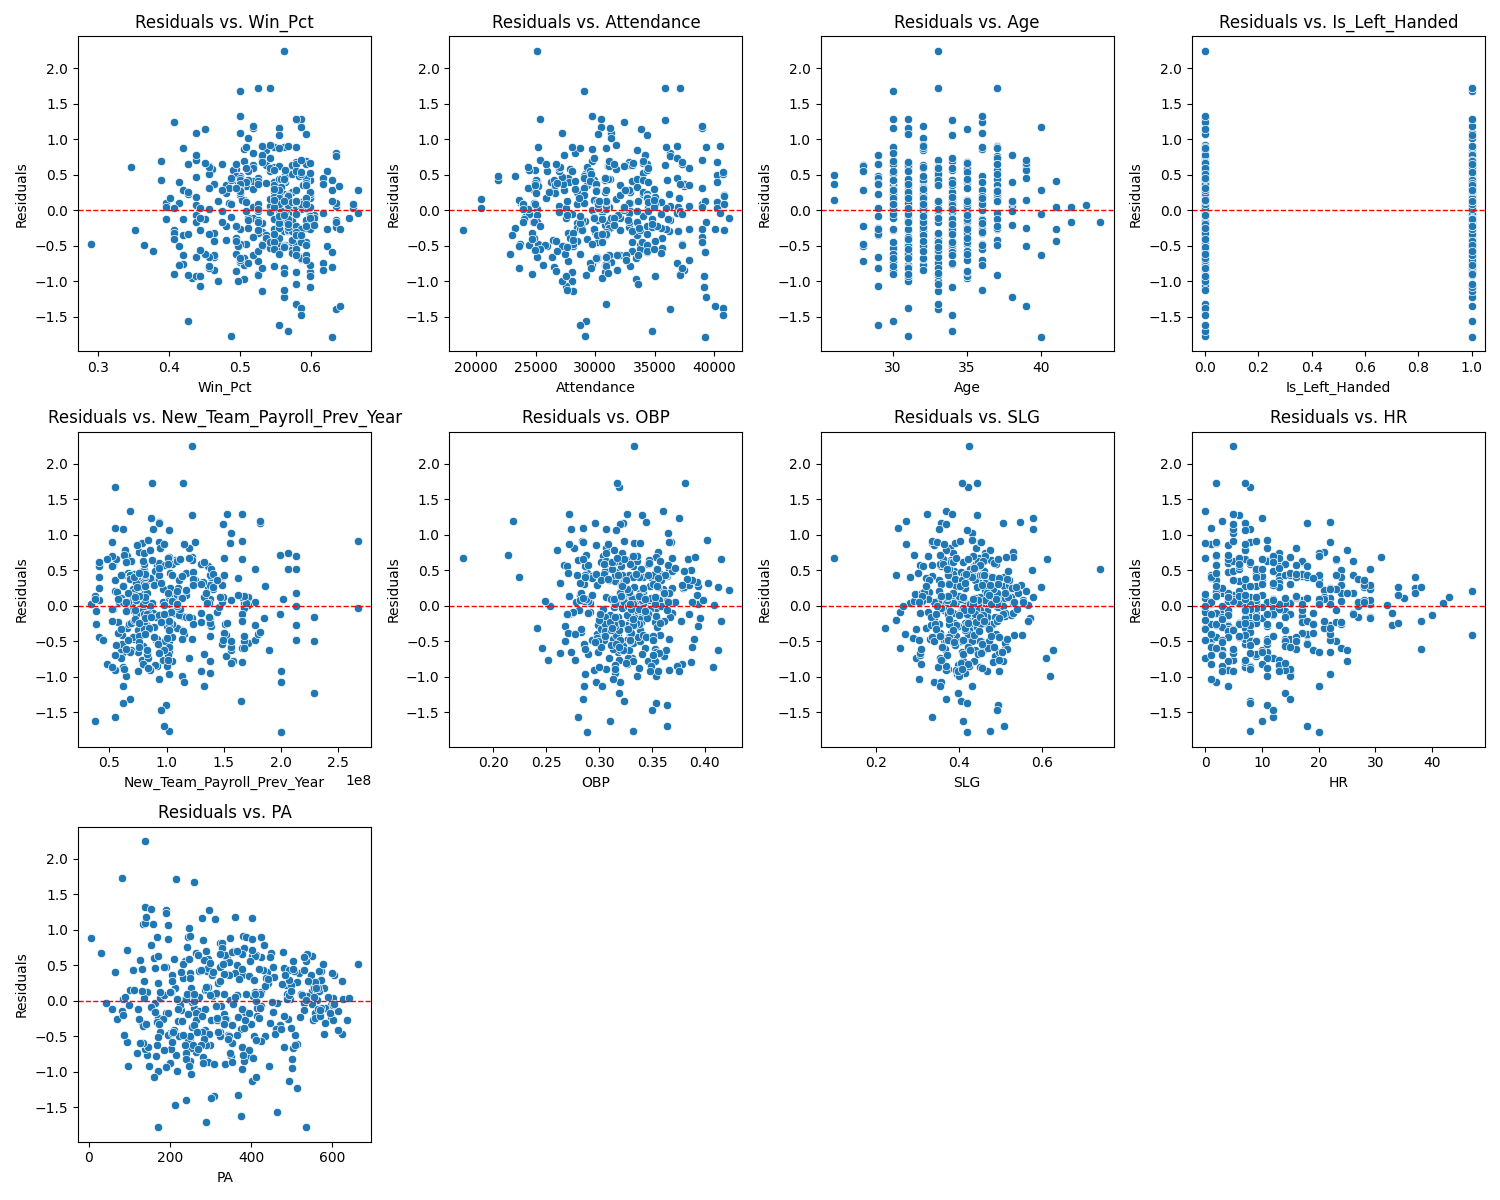
\includegraphics[height=0.75\textheight,keepaspectratio]{images/mlb_hitters_residuals.png}
    \end{block}
\end{frame}

\begin{frame}
    \frametitle{Results}
    \begin{block}{MLB Pitchers: Regression Results}
        \begin{table}[ht]
            \centering
            \caption{\( R^2 = 0.574 \)}
            \begin{tabular}{lcccc}
                \toprule
                Variable & Coeff. & Std. Err & t-value & $P > |t|$ \\
                \midrule
                \rowcolor{red!20} Win\_Pct & 7.048e+06 & 2.83e+06 & 2.491 & 0.013 \\
                \rowcolor{red!20} Attendance & 88.5332 & 37.329 & 2.372 & 0.018 \\
                \rowcolor{red!20} Age & -2.811e+05 & 5.34e+04 & -5.268 & 0.000 \\
                Is\_Left\_Handed & 2.667e+05 & 3.83e+05 & 0.697 & 0.486 \\
                \rowcolor{red!20} New\_Team\_Payroll\_Prev\_Year & 0.0129 & 0.004 & 3.201 & 0.001 \\
                ERA & -3.952e+04 & 1.79e+05 & -0.220 & 0.826 \\
                \rowcolor{red!20} WHIP & -4.003e+06 & 1.02e+06 & -3.934 & 0.000 \\
                \rowcolor{red!20} SO & 8.881e+04 & 8946.064 & 9.927 & 0.000 \\
                \rowcolor{red!20} IP & -1.962e+04 & 7618.119 & -2.576 & 0.010 \\
                \bottomrule
            \end{tabular}
        \end{table}        
    \end{block}
\end{frame}
\begin{frame}
    \frametitle{Results}
    \begin{block}{MLB Pitchers: Residuals}
        \centering
        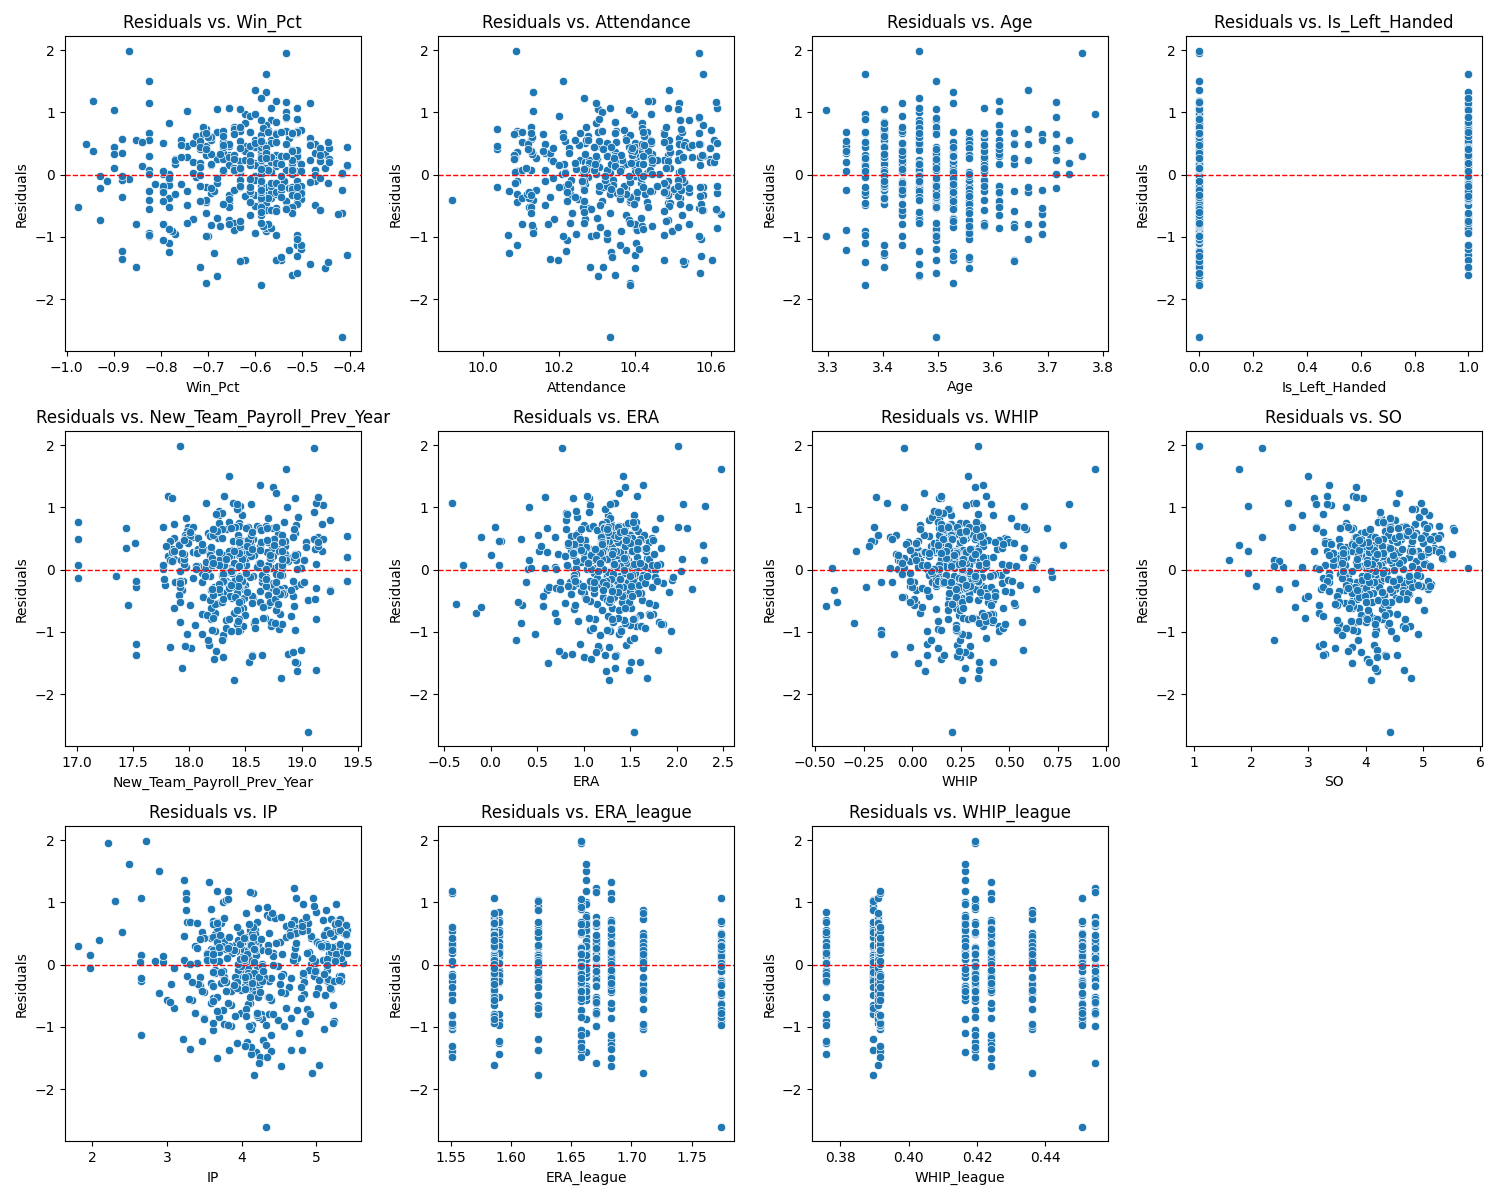
\includegraphics[height=0.75\textheight,keepaspectratio]{images/mlb_pitchers_residuals.png}
    \end{block}
\end{frame}

\begin{frame}
    \frametitle{Results}
    \begin{block}{KBO Hitters: Regression Results}
        \begin{table}[ht]
            \centering
            \caption{ \( R^2 = 0.481 \)}
            \begin{tabular}{lcccc}
            \toprule
            Variable & Coeff. & Std. Err & t-value & $P > |t|$ \\
            \midrule
            Win\_Pct & 0.5207 & 0.943 & 0.552 & 0.582 \\
            Attendance & 1.662e-07 & 2.34e-07 & 0.712 & 0.479 \\
            \rowcolor{red!20} Age & -0.0783 & 0.025 & -3.137 & 0.002 \\
            Is\_Left\_Handed & -0.0524 & 0.161 & -0.325 & 0.746 \\
            \rowcolor{red!20} OBP & 5.4557 & 2.346 & 2.325 & 0.023 \\
            SLG & -0.0155 & 1.255 & -0.012 & 0.990 \\
            HR & 0.0106 & 0.014 & 0.754 & 0.453 \\
            \rowcolor{red!20} PA & 0.0019 & 0.001 & 2.955 & 0.004 \\
            \bottomrule
            \end{tabular}
        \end{table}        
    \end{block}
\end{frame}

\begin{frame}
    \frametitle{Results}
    \begin{block}{KBO Hitters: Residuals}
        \centering
        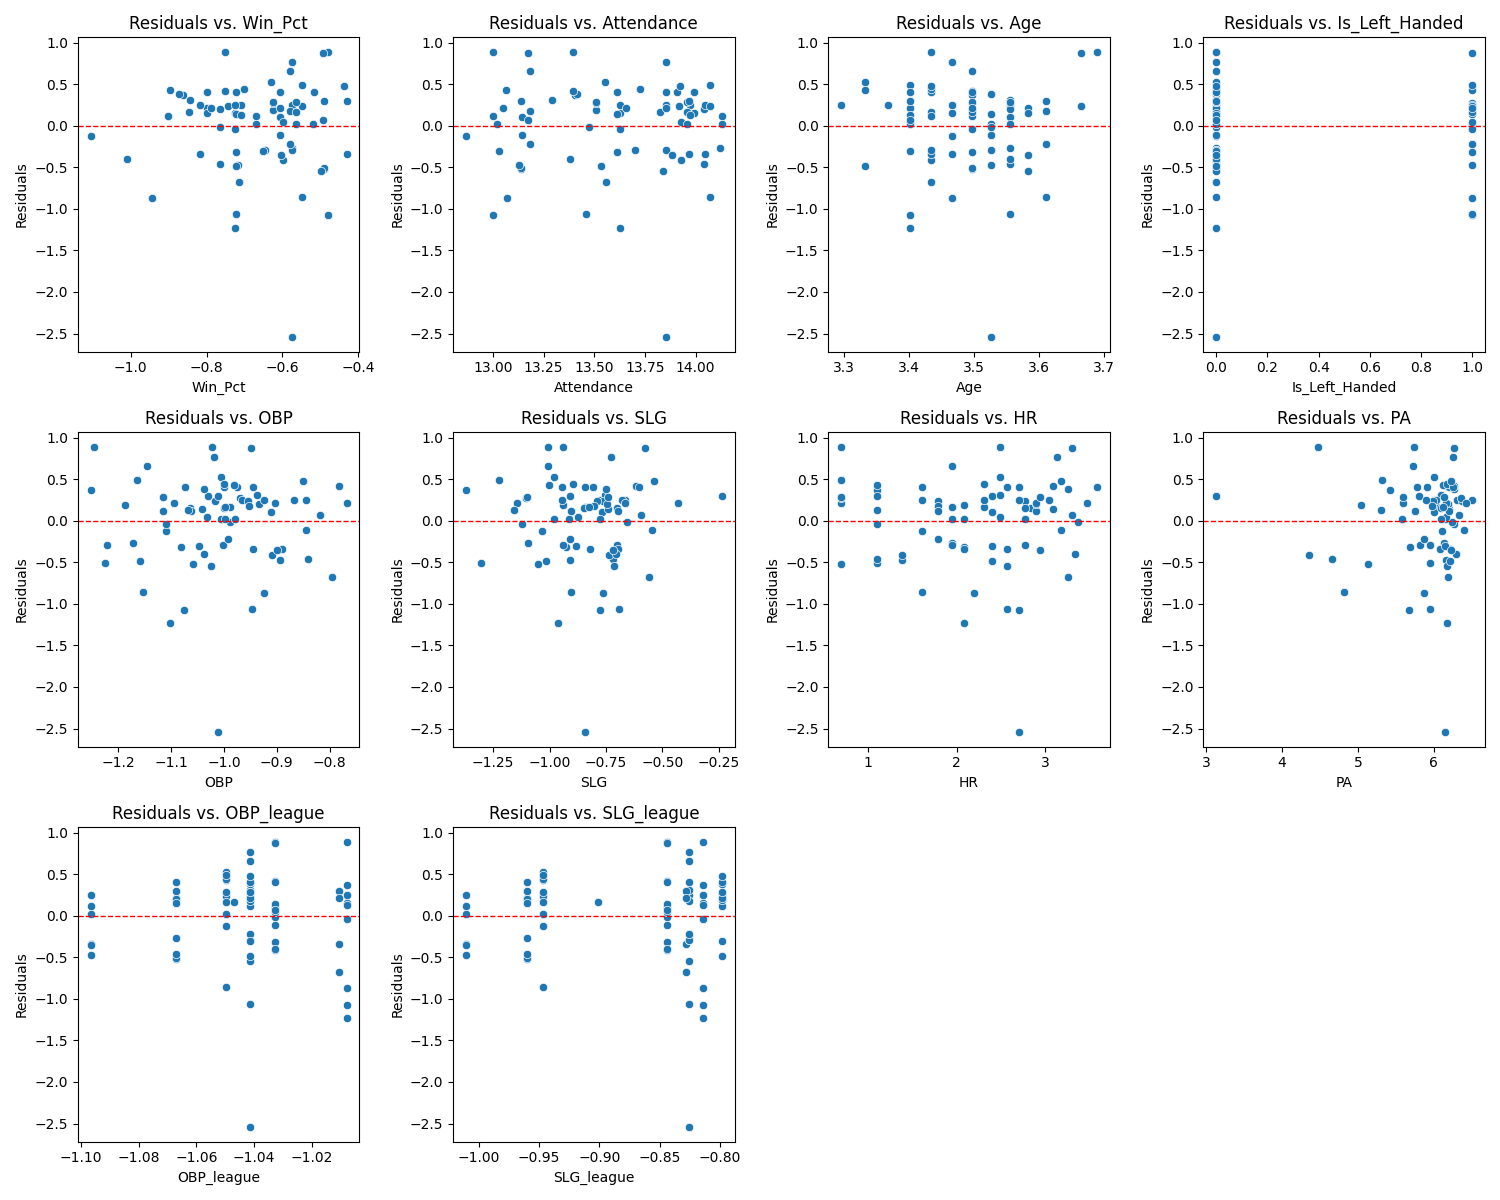
\includegraphics[width=0.9\textwidth,keepaspectratio]{images/kbo_hitters_residuals.png}
    \end{block}
\end{frame}

\begin{frame}
    \frametitle{Results}
    \begin{block}{KBO Pitchers: Regression Results}
        \begin{table}[ht]
            \centering
            \caption{\( R^2 = 0.321\)}
            \begin{tabular}{lcccc}
            \toprule
            Variable & Coeff. & Std. Err & t-value & $P > |t|$ \\
            \midrule
            Win\_Pct & 1.4626 & 1.534 & 0.953 & 0.346 \\
            Attendance & -3.153e-07 & 4.29e-07 & -0.734 & 0.467 \\
            \rowcolor{blue!20} Age & -0.0932 & 0.048 & -1.930 & 0.061 \\
            Is\_Left\_Handed & -0.2123 & 0.232 & -0.916 & 0.365 \\
            ERA & 0.0453 & 0.108 & 0.419 & 0.678 \\
            WHIP & -0.4594 & 0.841 & -0.546 & 0.588 \\
            \rowcolor{blue!20} SO & 0.0155 & 0.008 & 1.865 & 0.069 \\
            IP & -0.0064 & 0.006 & -1.020 & 0.314 \\
            \bottomrule
            \end{tabular}
        \end{table}               
    \end{block}
\end{frame}

\begin{frame}
    \frametitle{Results}
    \begin{block}{KBO Pitchers: Residuals}
        \centering
        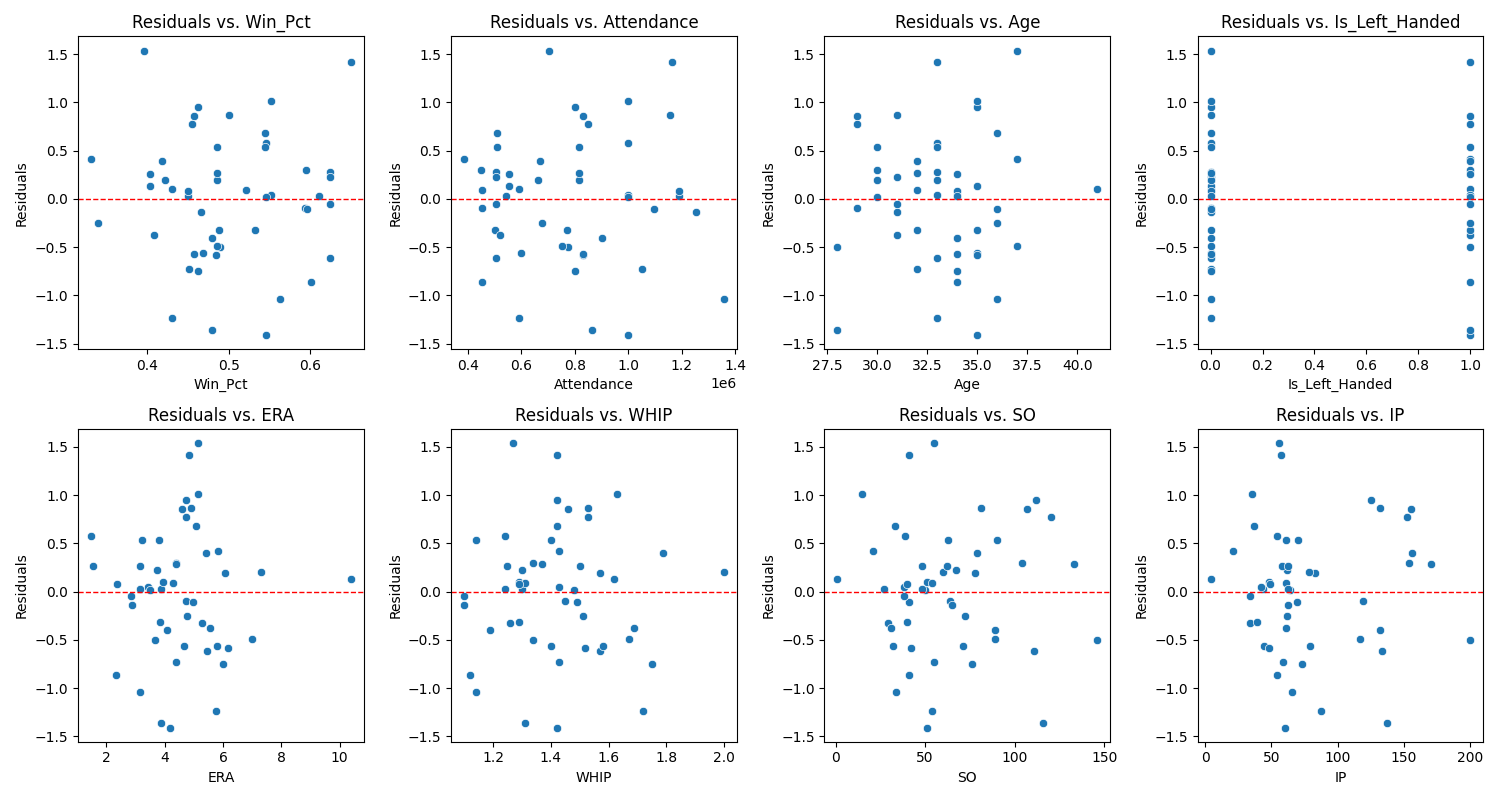
\includegraphics[width=0.9\textwidth,keepaspectratio]{images/kbo_pitchers_residuals.png}
    \end{block}
\end{frame}

\section{Discussion}
\begin{frame}
    \frametitle{Discussion}
    \begin{block}{Observations}
        \begin{itemize}
            \item In MLB, there was a clear sign of premium on playing in a team with higher win rate and home game attendance. This was not observed in KBO.
            \item In MLB the tendency of rich teams paying more was observed, which fits well with the common sense.
            \item In every set of data age negatively affected the AAV, which is consistent with the common sense.
            \item Unlike the common sense, being left-handed did not affect significantly to the AAV in any of the data.
            \item Except for the case of pitchers at KBO, playing more for team (higher PA and IP) in the previous season increased the AAV.
            \item $R^2$ were relatively higher in MLB than in KBO, which may be due to the difference in the size of market and pool of players. The supply in KBO is much smaller than in MLB, which may gives players more bargaining power and leads to stickier demand, resulting in more noise in the data.
        \end{itemize}
    \end{block}
\end{frame}

\begin{frame}
    \frametitle{Discussion}
    \begin{block}{Limitations}
        \begin{itemize}
            \item As breifly mentioned in the disclaimer, portion of samples were removed due to missing values, especially those who failed to find a team or from other leagues. To address this issue we need to adopt Tobit model, however it is beyound the scope of this project.
            \item To improve the model we tried with more variables such as league averages of performance factors, but there was no dramatic improvement in the $R^2$.
            \item Almost certainly there may be an endogeneity problem. However we could not come up with a good instrument variable to address this issue. Actually the league averages were initially considered as IV candidate but it turned out that in some cases their effect on AAV was significant.
            \item We only considered the factors related to batting for hitters, and pitching for pitchers. There may be other factors that affect the AAV, such as fielding, base running, or even personality. However these factors are hard to quantify, and the debate on effectiveness of current factors on these abilities is still ongoing.
        \end{itemize}
        
    \end{block}
\end{frame}

% \section{Conclusion}
% \begin{frame}
%     \frametitle{Conclusion}
% \end{frame}

\section{Appedices}

\begin{frame}
    \frametitle{Appendices: Actual vs. Fitted Values}
    \begin{block}{MLB Hitters}
        \centering
        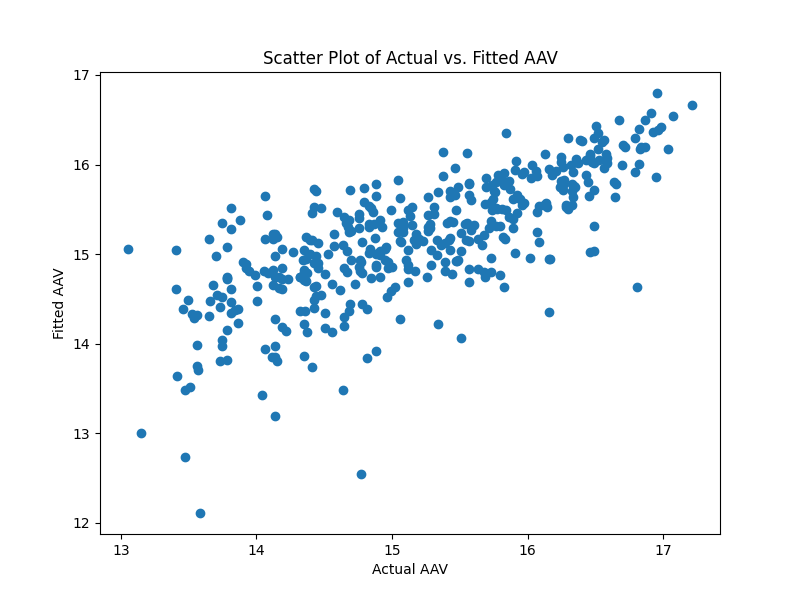
\includegraphics[width=0.9\textwidth,keepaspectratio]{images/mlb_hitters_fitted.png}
    \end{block}
\end{frame}

\begin{frame}
    \frametitle{Appendices: Actual vs. Fitted Values}
    \begin{block}{MLB Pitchers}
        \centering
        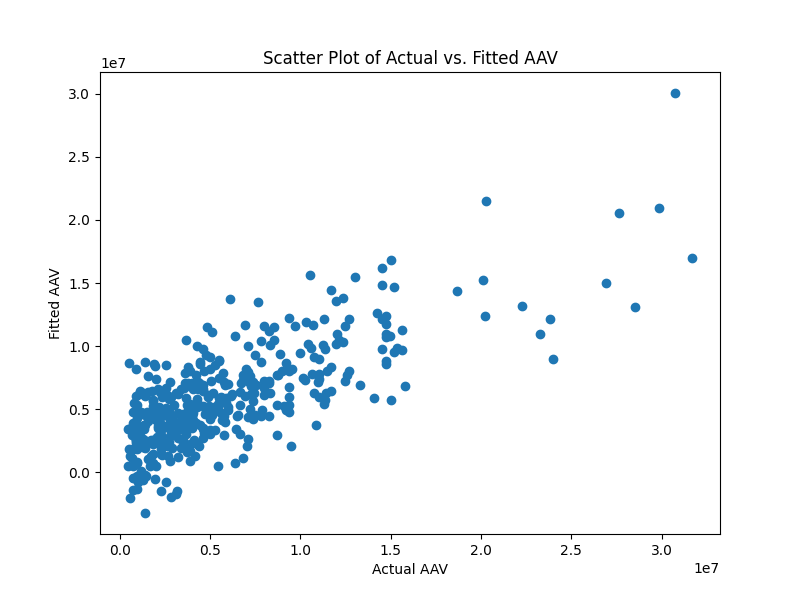
\includegraphics[width=0.9\textwidth,keepaspectratio]{images/mlb_pitchers_fitted.png}
    \end{block}
\end{frame}

\begin{frame}
    \frametitle{Appendices: Actual vs. Fitted Values}
    \begin{block}{KBO Hitters}
        \centering
        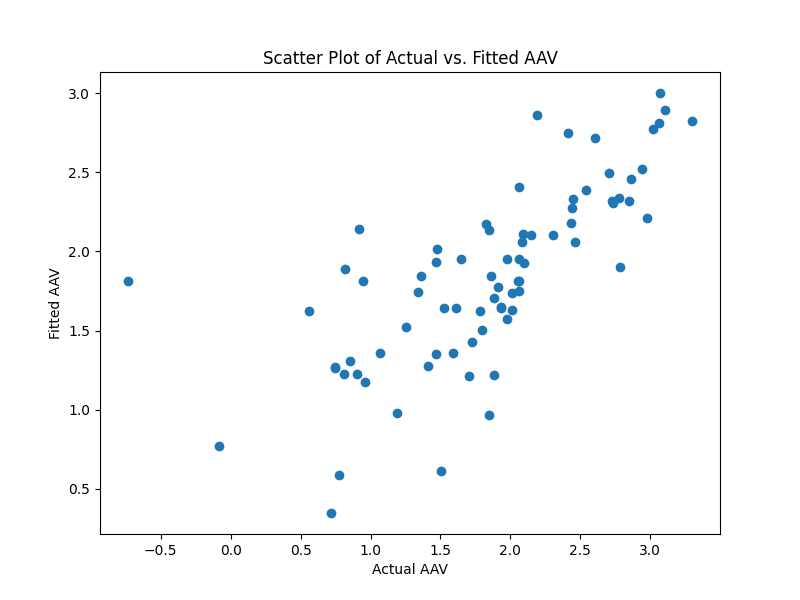
\includegraphics[width=0.9\textwidth,keepaspectratio]{images/kbo_hitters_fitted.png}
    \end{block}
\end{frame}

\begin{frame}
    \frametitle{Appendices: Actual vs. Fitted Values}
    \begin{block}{KBO Pitchers}
        \centering
        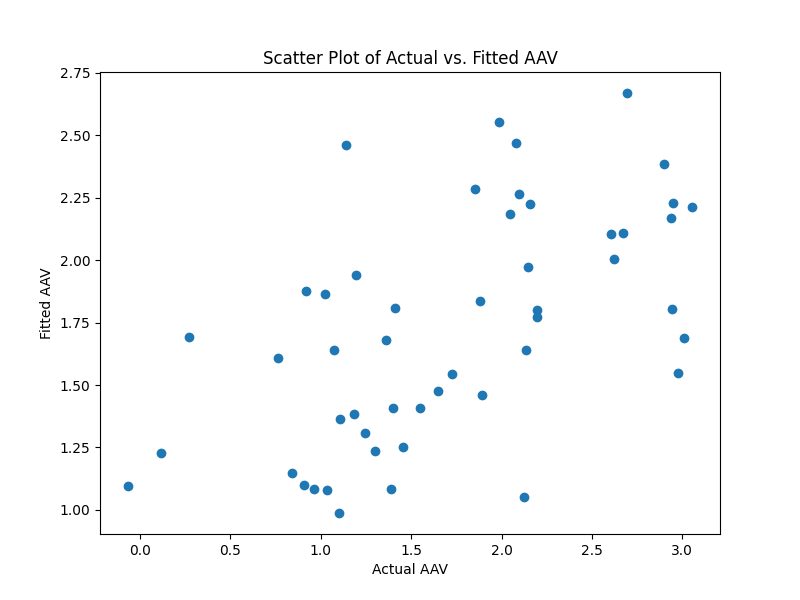
\includegraphics[width=0.9\textwidth,keepaspectratio]{images/kbo_pitchers_fitted.png}
    \end{block}
\end{frame}

\begin{frame}
    \frametitle{Appendices: Results with League Averages} 
    \begin{block}{MLB Hitters: Regression Results with League Averages}
        \begin{table}[ht]
            \centering
            \caption{$R^2 = 0.605$}
            \begin{tabular}{lcccc}
            \toprule
            Variable & Coeff. & Std. Err & t-value & $P > |t|$ \\
            \midrule
            \rowcolor{red!20} Win\_Pct & 1.6263 & 0.502 & 3.239 & 0.001 \\
            \rowcolor{red!20} Attendance & 1.862e-05 & 7.01e-06 & 2.657 & 0.008 \\
            \rowcolor{red!20} Age & -0.0592 & 0.011 & -5.595 & 0.000 \\
            Is\_Left\_Handed & -0.0921 & 0.060 & -1.528 & 0.127 \\
            \rowcolor{red!20} New\_Team\_Payroll\_Prev\_Year & 1.853e-09 & 7.41e-10 & 2.501 & 0.013 \\
            \rowcolor{red!20} OBP & 3.8651 & 1.174 & 3.294 & 0.001 \\
            \rowcolor{red!20} SLG & 1.8652 & 0.750 & 2.489 & 0.013 \\
            \rowcolor{red!20} HR & 0.0169 & 0.006 & 2.650 & 0.008 \\
            \rowcolor{red!20} PA & 0.0025 & 0.000 & 8.080 & 0.000 \\
            \rowcolor{red!20} OBP\_league & -19.3355 & 7.653 & -2.527 & 0.012 \\
            SLG\_league & -0.8215 & 3.344 & -0.246 & 0.806 \\
            \bottomrule
            \end{tabular}
        \end{table}
        
    \end{block}
\end{frame}

\begin{frame}
    \frametitle{Appendices: Results with League Averages} 
    \begin{block}{MLB Pitchers: Regression Results with League Averages}
        \begin{table}[ht]
            \centering
            \caption{$R^2 = 0.576$}
            \begin{tabular}{lcccc}
            \toprule
            Variable & Coeff. & Std. Err & t-value & $P > |t|$ \\
            \midrule
            \rowcolor{red!20} Win\_Pct & 7.93e+06 & 2.89e+06 & 2.746 & 0.006 \\
            \rowcolor{red!20} Attendance & 79.3230 & 37.817 & 2.098 & 0.037 \\
            \rowcolor{red!20} Age & -2.814e+05 & 5.36e+04 & -5.255 & 0.000 \\
            Is\_Left\_Handed & 2.745e+05 & 3.83e+05 & 0.717 & 0.474 \\
            \rowcolor{red!20} New\_Team\_Payroll\_Prev\_Year & 0.0132 & 0.004 & 3.260 & 0.001 \\
            ERA & -3419.6405 & 1.83e+05 & -0.019 & 0.985 \\
            \rowcolor{red!20} WHIP & -4.144e+06 & 1.03e+06 & -4.026 & 0.000 \\
            \rowcolor{red!20} SO & 9.107e+04 & 9161.492 & 9.940 & 0.000 \\
            \rowcolor{red!20} IP & -2.151e+04 & 7766.334 & -2.770 & 0.006 \\
            ERA\_league & -4.497e+05 & 1.03e+06 & -0.438 & 0.661 \\
            WHIP\_league & -3.289e+06 & 8.26e+06 & -0.398 & 0.691 \\
            \bottomrule
            \end{tabular}
        \end{table}
    \end{block}
\end{frame}

\begin{frame}
    \frametitle{Appendices: Results with League Averages} 
    \begin{block}{KBO Hitters: Regression Results with League Averages}
        \begin{table}[ht]
            \centering
            \caption{$R^2 = 0.493$}
            \begin{tabular}{lcccc}
            \toprule
            Variable & Coeff. & Std. Err & t-value & $P > |t|$ \\
            \midrule
            Win\_Pct & 0.6103 & 0.948 & 0.644 & 0.522 \\
            Attendance & 9.084e-08 & 2.47e-07 & 0.367 & 0.715 \\
            \rowcolor{red!20} Age & -0.0805 & 0.026 & -3.088 & 0.003 \\
            Is\_Left\_Handed & -0.0551 & 0.165 & -0.334 & 0.739 \\
            \rowcolor{blue!20} OBP & 4.4894 & 2.490 & 1.803 & 0.076 \\
            SLG & 0.3250 & 1.311 & 0.248 & 0.805 \\
            HR & 0.0136 & 0.014 & 0.949 & 0.346 \\
            \rowcolor{red!20} PA & 0.0021 & 0.001 & 3.063 & 0.003 \\
            OBP\_league & 10.7843 & 14.482 & 0.745 & 0.459 \\
            SLG\_league & -5.3348 & 4.333 & -1.231 & 0.222 \\
            \bottomrule
            \end{tabular}
        \end{table}
        
    \end{block}
\end{frame}

\begin{frame}
    \frametitle{Appendices: Results with League Averages} 
    \begin{block}{KBO Pitchers: Regression Results with League Averages}
        \begin{table}[ht]
            \centering
            \caption{$R^2 = 0.354$}
            \begin{tabular}{lcccc}
            \toprule
            Variable & Coeff. & Std. Err & t-value & $P > |t|$ \\
            \midrule
            Win\_Pct & 0.8255 & 1.625 & 0.508 & 0.614 \\
            Attendance & -4.22e-07 & 4.51e-07 & -0.936 & 0.355 \\
            Age & -0.0842 & 0.052 & -1.613 & 0.115 \\
            Is\_Left\_Handed & -0.2226 & 0.242 & -0.921 & 0.363 \\
            ERA & 0.0083 & 0.112 & 0.074 & 0.941 \\
            WHIP & -0.5786 & 0.846 & -0.684 & 0.498 \\
            SO & 0.0092 & 0.010 & 0.960 & 0.343 \\
            IP & -0.0041 & 0.007 & -0.613 & 0.544 \\
            ERA\_league & -0.0889 & 0.866 & -0.103 & 0.919 \\
            WHIP\_league & 3.5338 & 6.363 & 0.555 & 0.582 \\
            \bottomrule
            \end{tabular}
        \end{table}        
    \end{block}
\end{frame}

\end{document}